\documentclass[border=10pt]{standalone}

\usepackage{tikz}
\usepackage{tikzsymbols}
\usetikzlibrary{calc,patterns,shapes.geometric}

\def\centerarc[#1](#2)(#3:#4:#5){\draw[#1] ($(#2)+({#5*cos(#3)},{#5*sin(#3)})$) arc (#3:#4:#5);}

\begin{document}
	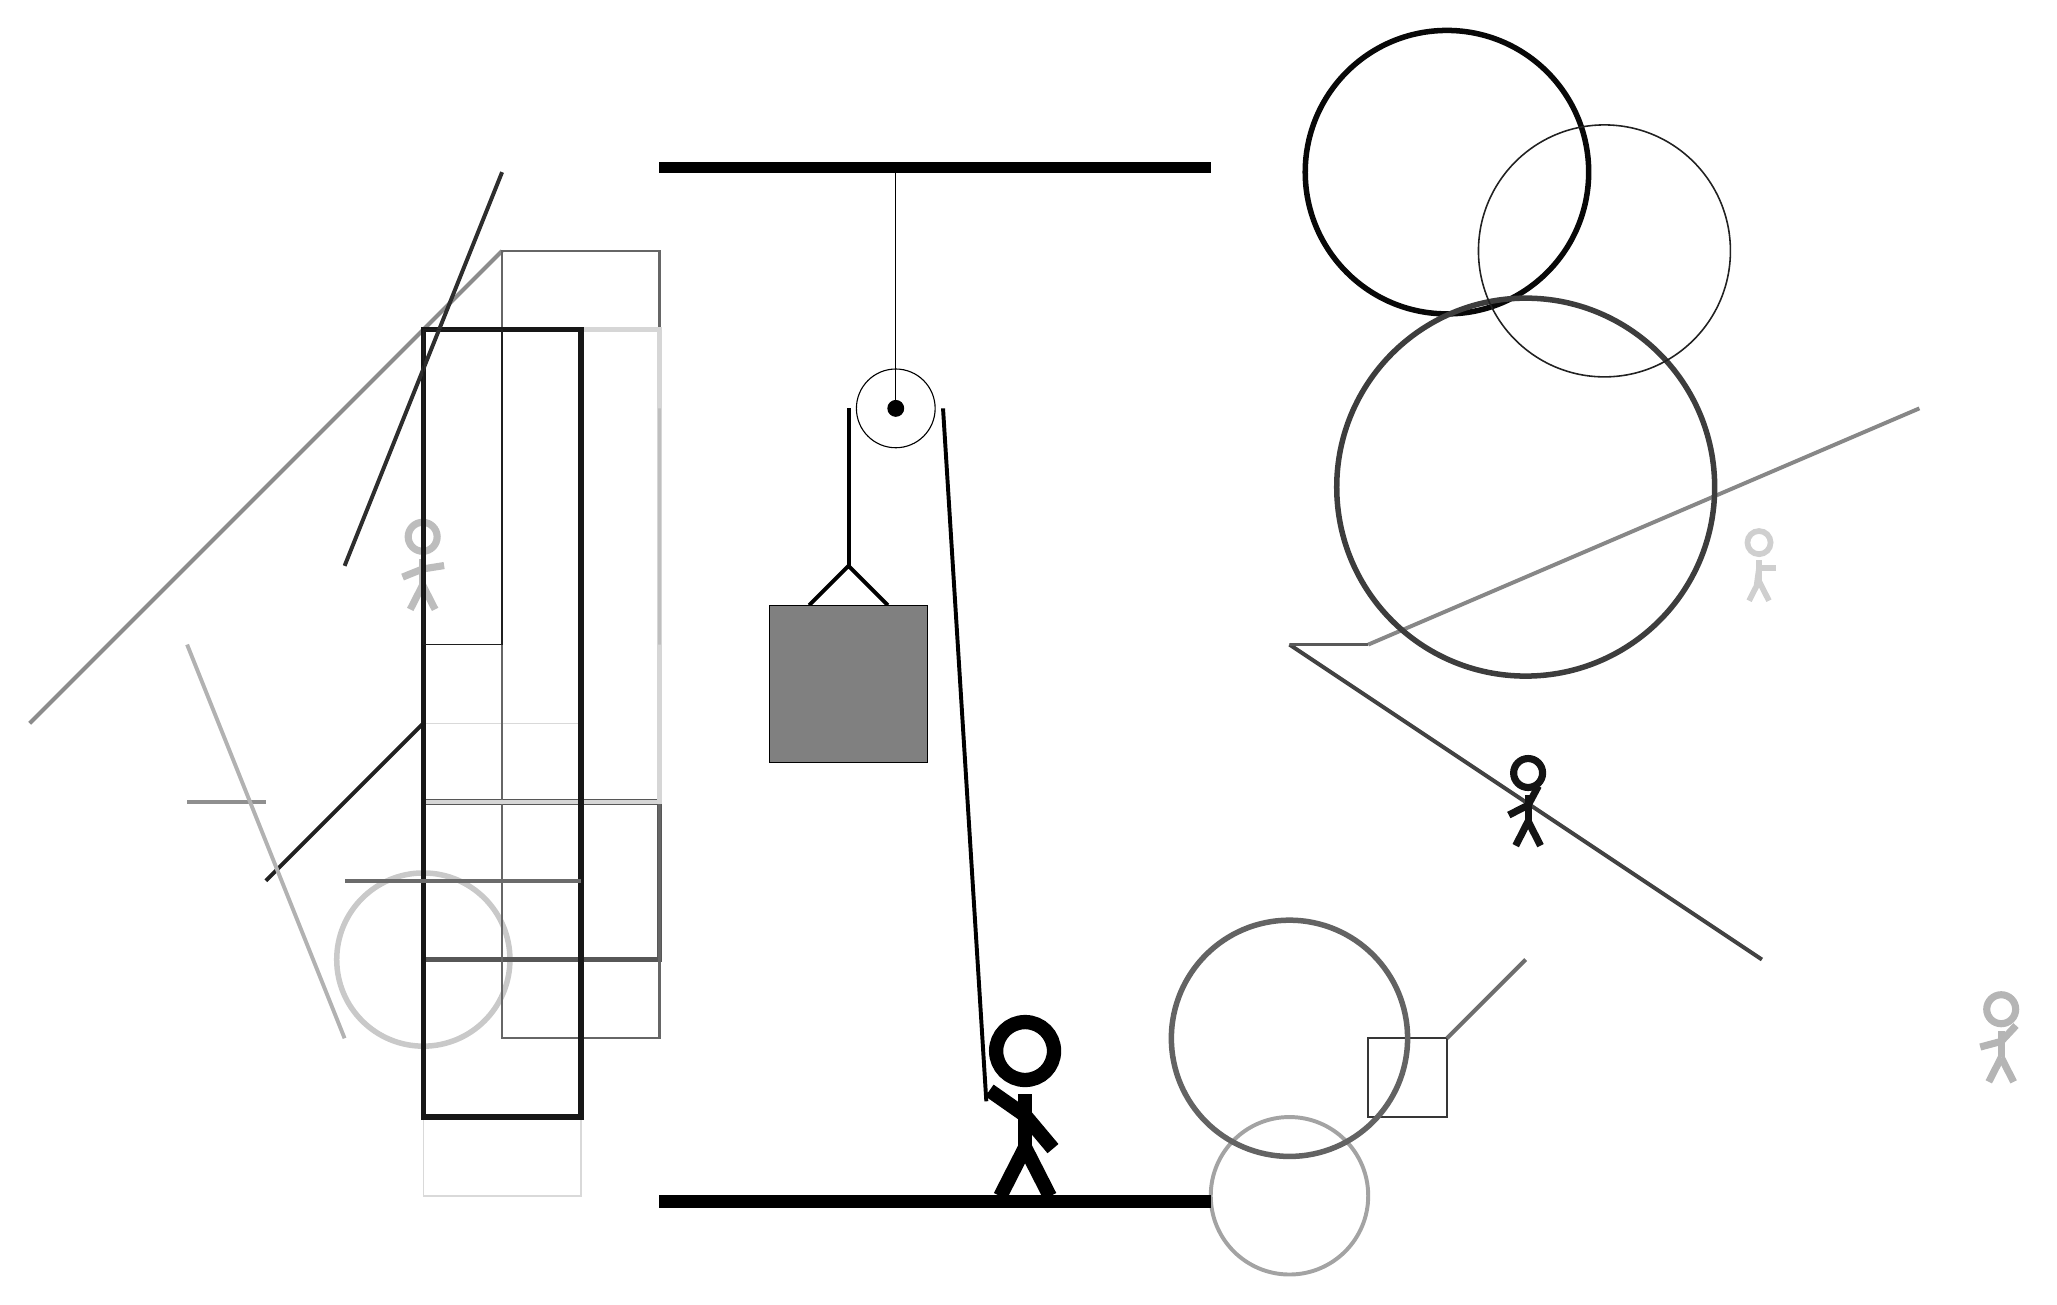
\begin{tikzpicture}
		%%%%% START %%%%%
		
		\draw[fill=black] (-2, 10) rectangle (5, 10.125);
		
		\draw (1, 7) circle (0.5);
		\draw[fill=black] (1, 7) circle (0.1);
		\draw (1, 10) -- (1, 7);
		
		\draw[line width=0.5mm] (-0.1, 4.5) -- (0.4, 5.0) -- (0.9, 4.5);
		\draw[fill=black!50] (-0.6, 4.5) rectangle (1.4, 2.5);
		
		\draw[line width=0.5mm] (0.4, 7) -- (0.4, 5.0);
		\centerarc[line width=0.5mm](1, 7)(0:180:0.6);
		\draw[line width=0.5mm](1.6, 7) -- (2.15, -1.8);
		
		\node at (2.6, -1.9) {\Strichmaxerl[10][-35][-50]};
		
		\node[line width=0.5mm, color=black!19] at (12, 5) {\Strichmaxerl[4][82][0]};
		
		\draw[line width=0.2mm, color=black!15] (-3, 3) rectangle (-5, -3);
		\draw[line width=0.5mm, color=black!47](7, 4) -- (14, 7);
		\draw [line width=0.7mm, color=black!21](-5, 0) circle (1.1);
		
		\draw[line width=0.5mm, color=black!45](-4, 9) -- (-10, 3);
		\draw[line width=0.3mm, color=black!79] (7, -1) rectangle (8, -2);
		\draw[line width=0.7mm, color=black!66] (-2, 2) rectangle (-5, 0);
		\node[line width=0.3mm, color=black!26] at (-5, 5) {\Strichmaxerl[5][22][9]};
		\draw [line width=0.7mm, color=black!97](8, 10) circle (1.8);
		\draw [line width=0.7mm, color=black!76](9, 6) circle (2.4);
		\node[line width=0.5mm, color=black!29] at (15, -1) {\Strichmaxerl[5][15][47]};
		
		\draw[line width=0.5mm, color=black!74](6, 4) -- (12, 0);
		\draw[line width=0.3mm, color=black!60] (-4, -1) rectangle (-2, 9);
		
		\draw[line width=0.5mm, color=black!57](9, 0) -- (8, -1);
		\draw[line width=0.6mm, color=black!16] (-2, 8) rectangle (-5, 2);
		\draw[line width=0.4mm, color=black!65] (6, 4) rectangle (7, 4);
		
		\draw[line width=0.5mm, color=black!44](-7, 2) -- (-8, 2);
		\draw [line width=0.5mm, color=black!36](6, -3) circle (1.0);
		\node[line width=0.7mm, color=black!92] at (9, 2) {\Strichmaxerl[5][27][62]};
		
		\draw[line width=0.5mm, color=black!87](-5, 3) -- (-7, 1);
		\draw[line width=0.7mm, color=black!91] (-3, 8) rectangle (-5, -2);
		\draw[line width=0.5mm, color=black!82](-4, 10) -- (-6, 5);
		
		\draw[line width=0.5mm, color=black!58](-3, 1) -- (-6, 1);
		\draw [line width=0.7mm, color=black!61](6, -1) circle (1.5);
		\draw[line width=0.3mm, color=black!25] (-2, 7) rectangle (-2, 4);
		\draw[line width=0.5mm, color=black!30](-6, -1) -- (-8, 4);
		\draw [line width=0.2mm, color=black!87](10, 9) circle (1.6);
		\draw[line width=0.2mm, color=black!88] (-4, 4) rectangle (-5, 8);
		
		\draw[fill=black] (-2, -3) rectangle (5, -3.15);
		
		%%%%% END %%%%%
	\end{tikzpicture}
\end{document}